%------------------------------------------------------------------------
% Chapter:  Examples
%------------------------------------------------------------------------

\chapter{Examples \label{exa}}

A simple example of the refinement of a single data set of $Ni$
was already given in section \ref{quick}. Here we will discuss
three slightly more complicated refinement examples. Some of the
example files are part of the tutorial found in the {\it PDFFIT}
distribution.

%------------------------------------------------------------------------

\section{Example 1: InGaAs\label{exa_gaas}}

In this section we will use $In_{0.5}Ga_{0.5}As$ to discuss the
question: What can be done when the first calculated PDF peak is
not sharp enough compared to the data ? \par

Figure \ref{exa_fig1a} shows the result of a straight forward
refinement of $In_{0.5}Ga_{0.5}As$ data. These data were collected
by V. Petvok and I.-K. Jeong at Cornell High Energy Synchrotron
Source. The maximum $Q$ value of these data is
$Q_{max}=45$\AA$^{-1}$. The corresponding macro file is listed
below. As usual we have added line numbers for convenience.

\begin{figure}[!htb]
   \centering
   \includegraphics[scale=0.65, angle=0]{exa.1a.eps}
   \caption[Result of PDF refinement A of $In_{0.5}Ga_{0.5}As$]
           {Result of PDF refinement A of $In_{0.5}Ga_{0.5}As$.
            The solid line is the calculated PDF, the filled circles are
            the data. Panel (a) shows the region around the split first
            PDF peak and (b) shows the complete refinement range.
            A difference curve is plotted below the data.}
   \label{exa_fig1a}
\end{figure}

\footnotesize
\begin{MacVerbatim}
      1 reset
      2 read stru,in50.stru
      3 read data,x,45.0,0.0,in50.data
      4 #
      5 urf 5.
      6 cyc 100
      7 range 1,1.5,10.0
\end{MacVerbatim}
\normalsize

\noindent First we reset {\it PDFFIT} (line 1), read the starting
structure (line 2) and the data (line 3). Our starting structure
includes static nearest neighbor displacements to account for the
different $In$-$As$ and $Ga$-$As$ bond length. The atom
coordinates of the starting structure are listed below:

\footnotesize
\begin{MacVerbatim}
   GA         -0.00500000       -0.00350000       -0.00350000
   IN          0.00550000        0.50550002        0.50550002
   GA          0.49450001       -0.00550000        0.49450001
   IN          0.50449997        0.50449997        0.00450000
   AS          0.26499999        0.23500000        0.26499999
   AS          0.26499999        0.76499999        0.73500001
   AS          0.75599998        0.26199999        0.73600000
   AS          0.73699999        0.76300001        0.23700000
\end{MacVerbatim}
\normalsize

\noindent As one can see, half of the metal sites are occupied by
$In$, the other half by $Ga$. All atoms have been shifted from
their ideal position to accommodate the static displacement. The
positions shown could be refined using {\it PDFFIT}, however, this
is beyond the scope of this section. In the next part we assign
parameters for the lattice parameters $a=b=c$ (line 13--15) and
corresponding starting values (lines 17--19). Next the scaling
factor, $\sigma_{Q}$ and the dynamic correlation factor $\delta$
are assigned to their refinement parameters (lines 21--23) and
again starting values for those parameters need to be given (lines
25--27).

\footnotesize
\begin{MacVerbatim}
      8 #
      9 ###############################################################
     10 # Experimental and lattice parameters
     11 ###############################################################
     12 #
     13 par lat[1]=p[1],1.0
     14 par lat[2]=p[1],1.0
     15 par lat[3]=p[1],1.0
     16 #
     17 p[1]=lat[1]
     18 p[2]=lat[1]
     19 p[3]=lat[1]
     20 #
     21 par csca[1]=p[20],1.0
     22 par qsig[1]=p[21],1.0
     23 par delt[1]=p[22],1.0
     24 #
     25 p[20]=0.40
     26 p[21]=0.03
     27 p[22]=0.10
\end{MacVerbatim}
\normalsize

\noindent In the next segment we assign two parameters for the
isotropic temperature factors $U=U_{11}=U_{22}=U_{33}$ for the
metal site occupied by $In$ and $Ga$ as well as for $As$. This is
done in a similar fashion than for the $Ni$ example given in
chapter \ref{quick} by using {\tt do} loops. A scan be seen from
the structure file shown above, the first four atoms are the
metals ($In,Ga$) and atoms 5 to 8 are $As$, so the first loop
(line 33) loops over atoms 1--4, the second loop goes over numbers
5--8.

\begin{figure}[!bth]
   \centering
   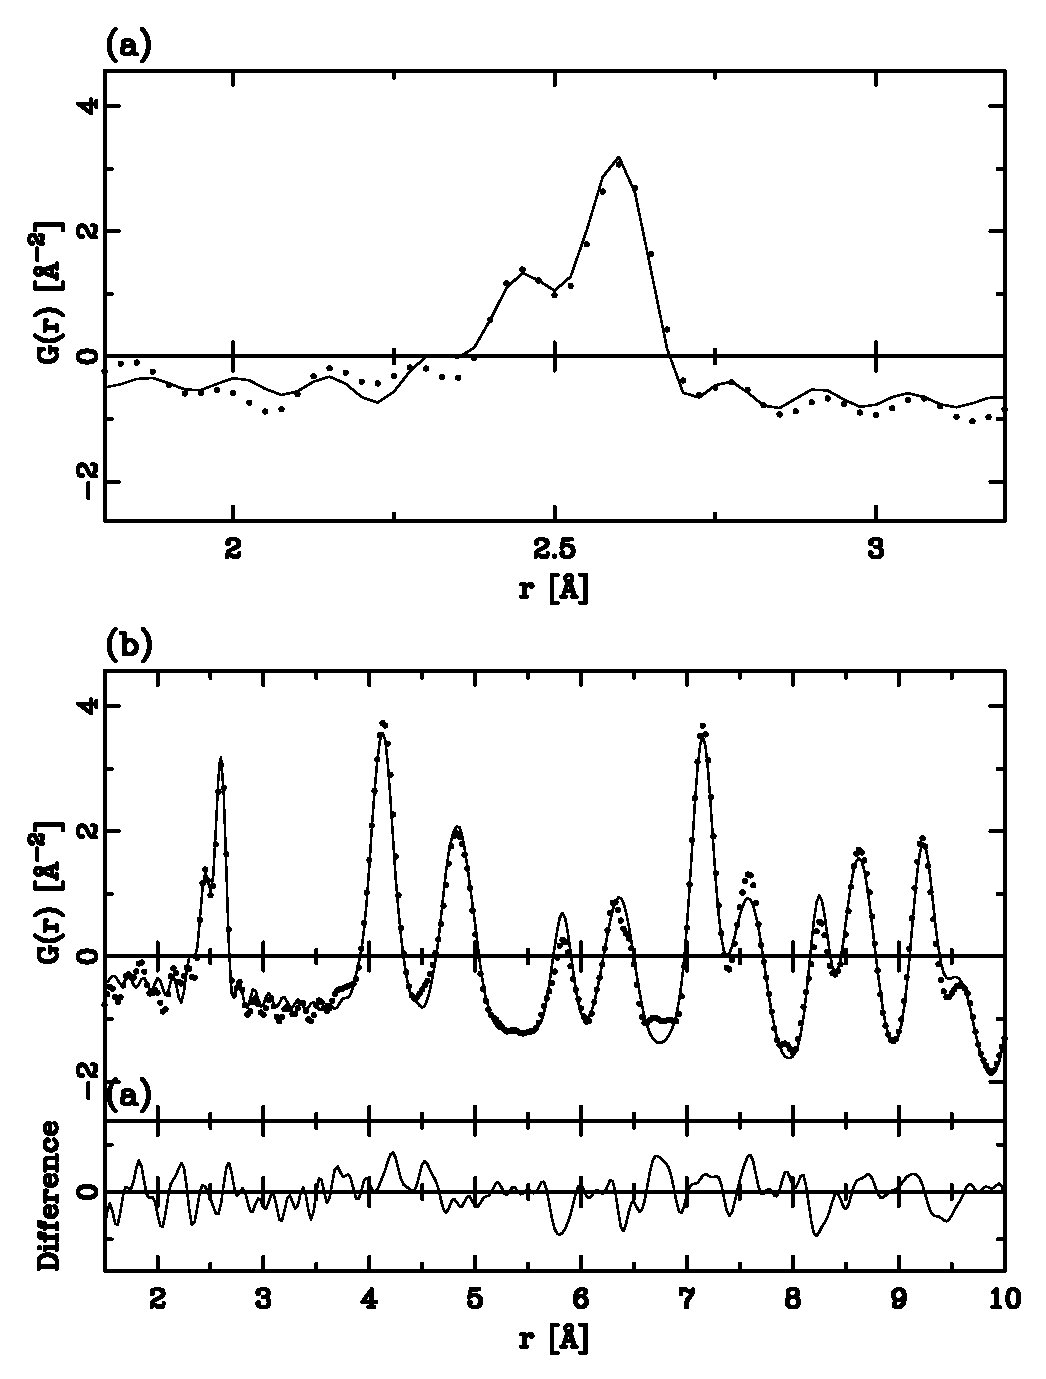
\includegraphics[scale=0.65, angle=0]{exa.1b.eps}
   \caption[Result of PDF refinement B of $In_{0.5}Ga_{0.5}As$]
           {Result of PDF refinement B of $In_{0.5}Ga_{0.5}As$.
            Details see caption of Figure \ref{exa_fig1a}.}
   \label{exa_fig1b}
\end{figure}

\footnotesize
\begin{MacVerbatim}
     28 #
     29 ###############################################################
     30 # Temperature factors
     31 ###############################################################
     32 #
     33 do i[1]=1,4
     34   par u[1,i[1]]=p[4],1.0
     35   par u[2,i[1]]=p[4],1.0
     36   par u[3,i[1]]=p[4],1.0
     37 enddo
     38 #
     39 do i[1]=5,8
     40   par u[1,i[1]]=p[5],1.0
     41   par u[2,i[1]]=p[5],1.0
     42   par u[3,i[1]]=p[5],1.0
     43 enddo
     44 #
     45 p[4]=u[1,1]
     46 p[5]=u[1,5]
\end{MacVerbatim}
\normalsize

\noindent After all parameter coding is done, we need to start the
refinement (line 47) and after the run is finished, we need to
save the results to individual files (lines 49--52).

\footnotesize
\begin{MacVerbatim}
     47 run
     48 #
     49 save pdf,1,in50.pdf
     50 save dif,1,in50.dif
     51 save stru,1,in50.rstr
     52 save res,in50.res
\end{MacVerbatim}
\normalsize

\noindent Inspection of Figure \ref{exa_fig1a} shows a reasonable
agreement when taking the complete $r$ range into account,
however, the split first neighbour peak shown in panel (a) of
Figure \ref{exa_fig1a} agrees rather badly with the observed PDF.
To understand this, we need to consider, that we have modeled
static displacements only for the nearest neighbour and
consequently only the width of the first PDF peak is completely
determined by thermal broadening whereas the other peaks are
determined by thermal as well as static displacements. The
dynamical correlation factor $\delta$ describes the $r$ dependence
of the PDF peak with according to the following empirical
equation:

\begin{equation}
  \sigma = \sigma` - \frac{\delta}{r^{2}}
\end{equation}

\noindent with $\sigma$ standing for the actual PDF peak width and
$\sigma'$ the width for uncorrelated motion, the value $\sigma$
converges to for high values of $r$. However, the parameter
$\delta$ is designed to take the correlated nature of thermal
motion into account. But in our case, we need a sharper transition
from the first peak which is purely thermal in origin and the
other peaks that contain thermal as well as static contributions.
To solve this problem, we sharpen the PDF peaks below a given
value $r_{cut}$ by a factor $\phi$ (see section \ref{fit_pwid} for
details. All we need to do, is to add the following lines to our
example macro:

\footnotesize
\begin{MacVerbatim}
     28a  par srat[1]=p[23],1.0
     28b  p[23]=0.3
     28c  rcut[1]=3.0
\end{MacVerbatim}
\normalsize

\noindent The ratio $\phi$ stored in the variable {\tt srat[s]} is
assigned to refinement parameter {\tt p[23]} (line 28a) and a
suitable starting value is set (line 28b). Furthermore, we need to
define the value of $r_{cut}$ or {\tt rcut[s]} for the
corresponding data set. This value determines below which value of
$r$ the PDF peak width is multiplied by $\phi$. The result of this
modified refinement can be seen in Figure \ref{exa_fig1b}. It is
obvious that the refinement describes the first PDF peak much
better, which is also reflected in the R-value of R=15.6\%
compared to R=19.1\% for the refinement without additional
sharpening.

%------------------------------------------------------------------------

\section{Example 2: Manganites\label{exa_mang}}

As a next example we will discuss a slightly more complicated
example, $LaMnO_{3}$. The structure is orthorhombic at room
temperature, space group $Pbnm$. Assuming one has an experimental
PDF, the first step is to obtain a starting structure. The data
used in this example were measured by G.H. Kwei and S.J.L.
Billinge on the special environment diffractometer (SEPD) at the
IPNS, Argonne. Unfortunately space group $Pbnm$ is a nonstandard
setting and the relations must be derived from space group $Pnma$
listed in the International Tables for Crystallography
\cite{tables} by cyclic permutation of the elements of the
relevant generators. Because we need this information later on,
the symmetrically equivalent positions are listed in Table
\ref{exa_tab2}.

\begin{table}[!htb]
\centering
\begin{tabular}{ccccc}
 (8d)& $x,y,z$
     & $x+\frac{1}{2},\overline{y}+\frac{1}{2},\overline{z}$
     & $\overline{x},\overline{y},z+\frac{1}{2}$
     & $\overline{x}+\frac{1}{2},y+\frac{1}{2},\overline{z}+\frac{1}{2}$
     \vspace{1mm} \\
     & $\overline{x},\overline{y},\overline{z}$
     & $\overline{x}+\frac{1}{2},y+\frac{1}{2},z$
     & $x,y,\overline{z}+\frac{1}{2}$
     & $x+\frac{1}{2},\overline{y}+\frac{1}{2},z+\frac{1}{2}$
     \vspace{2mm} \\
 (4c)& $x,y,\frac{1}{4}$
     & $x+\frac{1}{2},\overline{y}+\frac{1}{2},\frac{3}{4}$
     & $\overline{x},\overline{y},\frac{3}{4}$
     & $\overline{x}+\frac{1}{2},y+\frac{1}{2},\frac{1}{4}$
     \vspace{2mm} \\
 (4b)& $0,\frac{1}{2},0$
     & $\frac{1}{2},0,0$
     & $0,\frac{1}{2},\frac{1}{2}$
     & $\frac{1}{2},0,\frac{1}{2}$
\end{tabular}
\caption[Positions in space group $Pbnm$]
        {Symmetrically equivalent positions in space group $Pbnm$ for
         $Mn$ on (4b), $La,O$ on (4c) and $O$ on (8d).\label{exa_tab2}}
\end{table}

\noindent Using the same procedure as described in section
\ref{file_stru} we will use {\it DISCUS} to expand the structure
using the symmetry generators in space group $Pbnm$. The following
input file describes the structure as found in the literature
\citep{rohemo98}.

\footnotesize
\begin{MacVerbatim}
  title LaMnO3 - La (4c) - Mn (4b) - O (4c & 8d)
  spcgr Pbnm
  cell   5.5367   5.7473    7.6929   90.000000   90.000000   90.000000
  atoms
  LA         -0.007800        0.049000        0.250000     0.3400
  MN          0.000000        0.500000        0.000000     0.2100
  O           0.074500        0.487400        0.250000     0.5000
  O           0.725600        0.306600        0.038400     0.4300
\end{MacVerbatim}
\normalsize

\noindent Note that if we would use this structure file as input
for {\it PDFFIT} only those four atoms would be used. It is a
required step to use {\it DISCUS} to generate the other positions
or add them by hand. The expanded structure file that is used for
the refinement is shown below.

\footnotesize
\begin{MacVerbatim}
  title LaMnO3 - La (4c) - Mn (4b) - O (4c & 8d)
  spcgr Pbnm
  cell   5.5367   5.7473    7.6929   90.000000   90.000000   90.000000
  ncell        1,       1,       1,        20
  atoms
  LA           .992200         .049000         .250000      .3400
  LA           .492200         .451000         .750000      .3400
  LA           .007800         .951000         .750000      .3400
  LA           .507800         .549000         .250000      .3400
  MN           .000000         .500000         .000000      .2100
  MN           .500000         .000000         .000000      .2100
  MN           .000000         .500000         .500000      .2100
  MN           .500000         .000000         .500000      .2100
  O            .074500         .487400         .250000      .5000
  O            .574500         .012600         .750000      .5000
  O            .925500         .512600         .750000      .5000
  O            .425500         .987400         .250000      .5000
  O            .725600         .306600         .038400      .4300
  O            .225600         .193400         .961600      .4300
  O            .274400         .693400         .538400      .4300
  O            .774400         .806600         .461600      .4300
  O            .274400         .693400         .961600      .4300
  O            .774400         .806600         .038400      .4300
  O            .725600         .306600         .461600      .4300
  O            .225600         .193400         .538400      .4300
\end{MacVerbatim}
\normalsize

\noindent This structure file now contains all 20 atoms per unit
cell. Note that {\it DISCUS} could also have been used to create a
larger model structure, e.g. 2x1x1 unit cells. Note that per
convention {\it DISCUS} will transform the fractional coordinates
of all atoms within a single unit cell to the range 0 to 1. \par

After having the required input files, i.e. an experimental PDF and
a starting structure, one can start the refinement. In our example
we want to refine isotropic temperature factors as well as positions,
however, the symmetry constraints given by space group $Pbnm$ shall
be applied. The following sequence of commands is used for the refinement.
Obviously it is more convenient to prepare a text file with the commands
and start it as a macro in {\it PDFFIT} using the {\tt @} command. As before
the line numbers in the example here are for easy reference only and not
part of the actual input.

\footnotesize
\begin{MacVerbatim}
      1 reset
      2 read stru,lmo.stru
      3 read data,n,27.0,0.03,lmo.data
      4 #
      5 urf 5.0
      6 cyc 100
      7 range 1.0,15.0
\end{MacVerbatim}
\normalsize

\noindent After {\it PDFFIT} has been reset (line 1), the starting
structure (line 2) and PDF data (line 3) are read. The parameters
in line 3 identify the data to be obtained from neutron scattering
({\tt n}) with a maximum $Q$ value of $Q_{max}=27$\AA$^{-1}$. The
next parameters specifies the value for $\sigma_{Q}$ followed by
the name of the data file. For details about the file formats and
conversion tools refer to chapter \ref{file} of this manual. In
line 5 the magic number for the refinement is set to 5.0 (see
section \ref{fit_opt}). Next the maximum number of iterations is
set to 100, which is of course much larger than the number of
iteration we expect before the fit converges (or explodes). The
command {\tt range} (line 7) sets the range in real space used for
the refinement to 1.0 to 15.0\AA. The main part of the example
macro contains refinement parameter definitions. We start with
lattice parameters and some experimental parameters.

\footnotesize
\begin{MacVerbatim}
      8 #
      9 ###############################################################
     10 # Experimental and lattice parameters
     11 ###############################################################
     12 #
     13 par lat[1]=p[1],1.0
     14 par lat[2]=p[2],1.0
     15 par lat[3]=p[3],1.0
     16 #
     17 p[1]=lat[1]
     18 p[2]=lat[2]
     19 p[3]=lat[3]
     20 #
     21 par csca[1]=p[200],1.0
     22 par qsig[1]=p[201],1.0
     23 par delt[1]=p[202],1.0
     24 #
     25 p[200]=0.40
     26 p[201]=0.03
     27 p[202]=0.10
\end{MacVerbatim}
\normalsize

\noindent Lines 8--12 are simply a comment to make the macro file
easier to read. It is generally recommended to include descriptive
comments in refinement macros. Since our structure is
orthorhombic, we assign three parameters {\tt p[1],p[2]} and {\tt
p[3]} to refine the lattice parameters $a,b$ and $c$ stored in
variables {\tt lat[1], lat[2]} and {\tt lat[3]} (line 13--15). The
syntax of the command {\tt par} was already discussed in detail in
section \ref{fit_code}. The starting values for the parameters
{\tt p[1]} to {\tt p[3]} are set in lines 17--19. It is important
to assign each used refinement parameter a proper starting value
before starting the refinement. In lines 21--23 we assign
parameters to the scale factor $f_{p}$, the resolution parameter
$\sigma_{Q}$ and the dynamic correlation factor $\delta$. Again
each parameter needs a proper starting value (lines 25--27). The
choice which parameters {\tt p[n]} is assigned to which
experimental or structural parameter is completely up to the user.

\footnotesize
\begin{MacVerbatim}
     28 #
     29 ###############################################################
     30 # Temperature factors
     31 ###############################################################
     32 #
     33 do i[1]=1,4
     34   par u[1,i[1]]=p[4],1.0
     35   par u[2,i[1]]=p[4],1.0
     36   par u[3,i[1]]=p[4],1.0
     37 enddo
     38 #
     39 do i[1]=5,8
     40   par u[1,i[1]]=p[5],1.0
     41   par u[2,i[1]]=p[5],1.0
     42   par u[3,i[1]]=p[5],1.0
     43 enddo
     44 #
     45 p[4]=u[1,1]
     46 p[5]=u[1,5]
     47 #
     48 do i[1]=9,16
     49   par u[1,i[1]]=p[6],1.0
     50   par u[2,i[1]]=p[6],1.0
     51   par u[3,i[1]]=p[6],1.0
     52 enddo
     53 #
     54 do i[1]=17,20
     55   par u[1,i[1]]=p[7],1.0
     56   par u[2,i[1]]=p[7],1.0
     57   par u[3,i[1]]=p[7],1.0
     58 enddo
     59 #
     60 p[6]=u[1, 9]
     61 p[7]=u[1,17]
\end{MacVerbatim}
\normalsize

\noindent In out structure, we have atoms on four different
positions: $Mn$ on (4b), $La, O$ on (4c) and $O$ on (8d). The
program {\it PDFFIT} assigns numbers to each atom in the same
order they appear in the structure file. Inspecting the structure
file listed above, we find that atoms 1--4 are $Mn$, 5--8 are
$La$, 9--16 are the oxygens on position (4c) and finally atoms
17--20 are the oxygens on position (8d). The command sequence
above assigns an individual isotropic thermal parameter
$U=U_{11}=U_{22}=U_{33}$ to all four atom types (two for the
different oxygens). In this example we use {\tt do} loops for the
parameter assignment (see section \ref{fit_code}). The first loop
(line 33) goes over atoms 1 to 4 and assigns parameters {\tt
u[1,n], u[2,n]} and {\tt u[3,n]} a single refinement parameter
{\tt p[4]}. The same is done for the $La$ atoms in lines 39--43.
Next starting values are given to the parameters (lines 45--46).
The last part of this segment assigns isotropic temperature
factors to the two different oxygen sites in a similar way. \par

So far the example was quite straight forward and not really different
from the simple macro given in chapter \ref{quick}. Next we want to
refine the atom positions, but restricted to the space group $Pbnm$.
For $Mn$ we have no free positional parameter, for $La$ and oxygen on
position (4c) there are two refinable parameters $(x,y)$ and for
the oxygen on position (8d) all three coordinates can be refined.
The parameter coding for $La$ is show below:

\footnotesize
\begin{MacVerbatim}
     62 #
     63 ###############################################################
     64 # Positions (constrained)
     65 ###############################################################
     66 #
     67 # La on (4c)
     68 #
     69 par x[ 1]= 1.0+p[21], 1.0
     70 par y[ 1]= 0.0+p[22], 1.0
     71 par x[ 2]= 0.5+p[21], 1.0
     72 par y[ 2]= 0.5-p[22],-1.0
     73 par x[ 3]= 0.0-p[21],-1.0
     74 par y[ 3]= 1.0-p[22],-1.0
     75 par x[ 4]= 0.5-p[21],-1.0
     76 par y[ 4]= 0.5+p[22], 1.0
     77 #
     78 p[21]=-0.0078
     79 p[22]= 0.0490
\end{MacVerbatim}
\normalsize

\noindent The $x$ coordinate of atom one is assigned to parameter
{\tt p[21]} and $y$ is assigned {\tt p[22]}. In line 69 and 74 we
have added 1.0 to conform to the {\it DISCUS} convention that
fractional coordinates range from 0 to 1. The atom positions of
the other three $La$ atoms are calculated according to the
relations given in Table \ref{exa_tab2}. Note the sign of the
derivatives in this example ! The coding for the oxygens on site
(4c) is exactly the same (apart from $\pm$1.0) and shown below:

\footnotesize
\begin{MacVerbatim}
     80 #
     81 # O on (4c)
     82 #
     83 par x[ 9]=0.0+p[23], 1.0
     84 par y[ 9]=0.0+p[24], 1.0
     85 par x[10]=0.5+p[23], 1.0
     86 par y[10]=0.5-p[24],-1.0
     87 par x[11]=1.0-p[23],-1.0
     88 par y[11]=1.0-p[24],-1.0
     89 par x[12]=0.5-p[23],-1.0
     90 par y[12]=0.5+p[24], 1.0
     91 #
     92 p[23]= 0.0745
     93 p[24]= 0.4874
\end{MacVerbatim}
\normalsize

\noindent The coding for the oxygen atoms on site (8d) is slightly
longer since we change all three coordinates and have 8
symmetrically equivalent positions. However, following Table
\ref{exa_tab2} there should be no difficulty to understand the
following part of the {\it PDFFIT} macro.

\footnotesize
\begin{MacVerbatim}
     94 #
     95 # O on (8d)
     96 #
     97 par x[13]= 0.0+p[25], 1.0
     98 par y[13]= 0.0+p[26], 1.0
     99 par z[13]= 0.0+p[27], 1.0
    100 par x[14]=-0.5+p[25], 1.0
    101 par y[14]= 0.5-p[26],-1.0
    102 par z[14]= 1.0-p[27],-1.0
    103 par x[15]= 1.0-p[25],-1.0
    104 par y[15]= 1.0-p[26],-1.0
    105 par z[15]= 0.5+p[27], 1.0
    106 par x[16]= 1.5-p[25], 1.0
    107 par y[16]= 0.5+p[26], 1.0
    108 par z[16]= 0.5-p[27],-1.0
    109 par x[17]= 1.0-p[25],-1.0
    110 par y[17]= 1.0-p[26],-1.0
    111 par z[17]= 1.0-p[27],-1.0
    112 par x[18]= 1.5-p[25],-1.0
    113 par y[18]= 0.5+p[26], 1.0
    114 par z[18]= 0.0+p[27], 1.0
    115 par x[19]= 0.0+p[25], 1.0
    116 par y[19]= 0.0+p[26], 1.0
    117 par z[19]= 0.5-p[27],-1.0
    118 par x[20]=-0.5+p[25], 1.0
    119 par y[20]= 0.5-p[26],-1.0
    120 par z[20]= 0.5+p[27], 1.0
    121 #
    122 p[25]= 0.7256
    123 p[26]= 0.3066
    124 p[27]= 0.0384
\end{MacVerbatim}
\normalsize

\noindent Now the parameter coding is complete and the refinement
can be started using the command {\tt run} (line 125). After the
fit has converged, the results have to be stored. In line 127 the
resulting structure is saved to the file {\it lmo\_ref.stru}, next
the calculated PDF and its difference to the experimental data are
written to a file (lines 128--129) and finally the refinement
result is saved to the file {\it lmo\_ref.res}.

\footnotesize
\begin{MacVerbatim}
    125 run
    126 #
    127 save stru,1,lmo_ref.stru
    128 save pdf,1,lmo_ref.pdf
    129 save dif,1,lmo_ref.dif
    130 save res,lmo_ref.res
\end{MacVerbatim}
\normalsize

\begin{figure}[!bt]
   \centering
   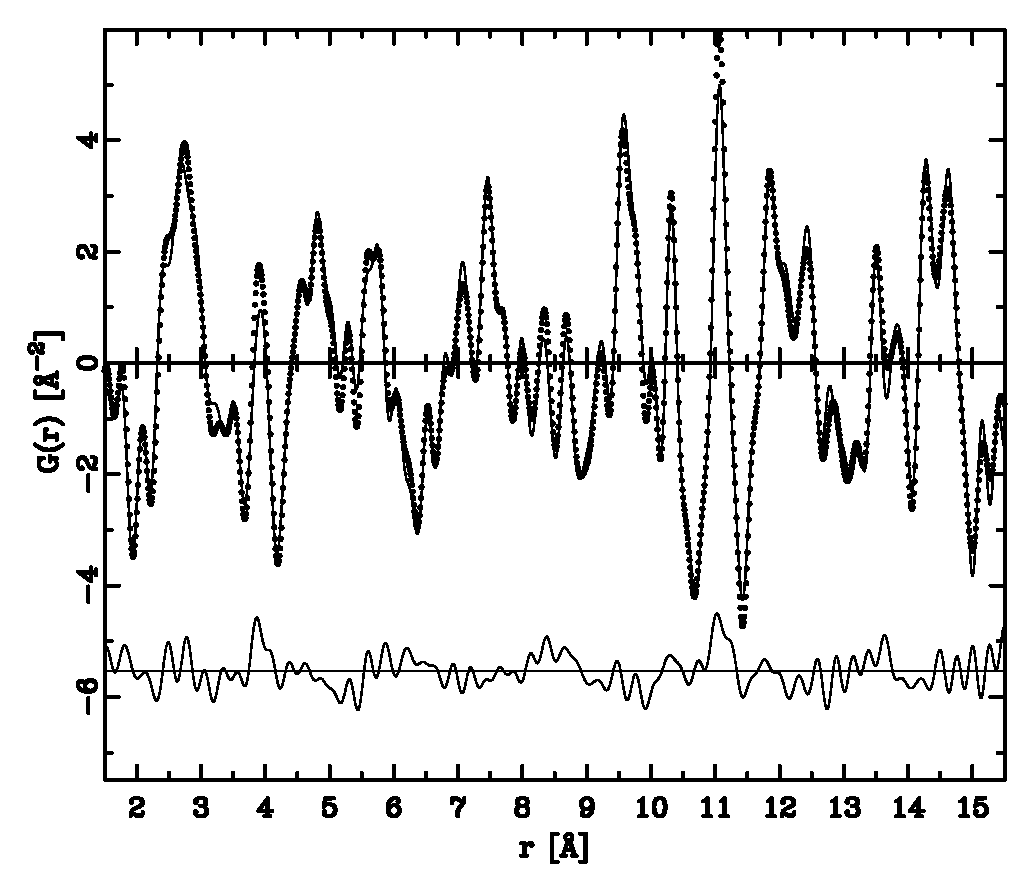
\includegraphics[scale=0.65, angle=0]{exa.2.eps}
   \caption[Result of PDF refinement of $LaMnO_{3}$]
           {Result of PDF refinement of $LaMnO_{3}$. The solid line is the
            calculated PDF, the filled circles are the data. A difference
            curve is plotted below the data.}
   \label{exa_fig2}
\end{figure}

\noindent The result of the refinement is shown in Figure
\ref{exa_fig2}. The next step one might be interested in is to
refine the positions of the oxygen atoms without the symmetry
restrictions imposed by space group $Pbnm$ since the $Mn-O$
octahedra might have {\it locally} a different symmetry. One way
of doing this is to construct different constraint equations based
on geometrical considerations. Alternatively one could refine all
oxygen coordinates individually. One possible parameter coding
shown below is quite similar to the coding of the thermal factors
above.

\footnotesize
\begin{MacVerbatim}
      1 ###############################################################
      2 # Positions O1 and O2 (free)
      3 ###############################################################
      4 do i[1]=9,12
      5   par x[i[1]]=p[i[1]*3+51],1.0
      6   par y[i[1]]=p[i[1]*3+52],1.0
      7 #
      8   p[i[1]*3+51]=x[i[1]]
      9   p[i[1]*3+52]=y[i[1]]
     10 enddo
     11 #
     12 do i[1]=13,20
     13   par x[i[1]]=p[i[1]*3+51],1.0
     14   par y[i[1]]=p[i[1]*3+52],1.0
     15   par z[i[1]]=p[i[1]*3+53],1.0
     16 #
     17   p[i[1]*3+51]=x[i[1]]
     18   p[i[1]*3+52]=y[i[1]]
     19   p[i[1]*3+53]=z[i[1]]
     20 enddo
\end{MacVerbatim}
\normalsize

\noindent Note that we are not refining the $z$ value of the
oxygen sitting on site (4c), although in principle one could try
even that. It is important to understand, that the PDF probes the
{\it local} structure. By selecting different ranges in $r$ one
has control over the length scale on which the refined {\it local}
arrangement occurs. For further reading refer to the references
given in the introduction of this users guide.

%------------------------------------------------------------------------

\section{Example 3: Nickel using multiple data sets\label{exa_nimul}}

In this section a combined refinement of two data sets for $Ni$
will be shown. The first data set was already used in the $Ni$
example shown in chapter \ref{quick} with a value of
$Q_{max}=22$\AA$^{-1}$. The second data set is taken from the
Billinge group (Michigan State University) diffractometer using a
conventional X-ray tube as source. Using MoK$\alpha$ radiation a
value of $Q_{max}=16$\AA$^{-1}$ could be reached. The refinement
macro file is listed below:

\begin{figure}[!tb]
   \centering
   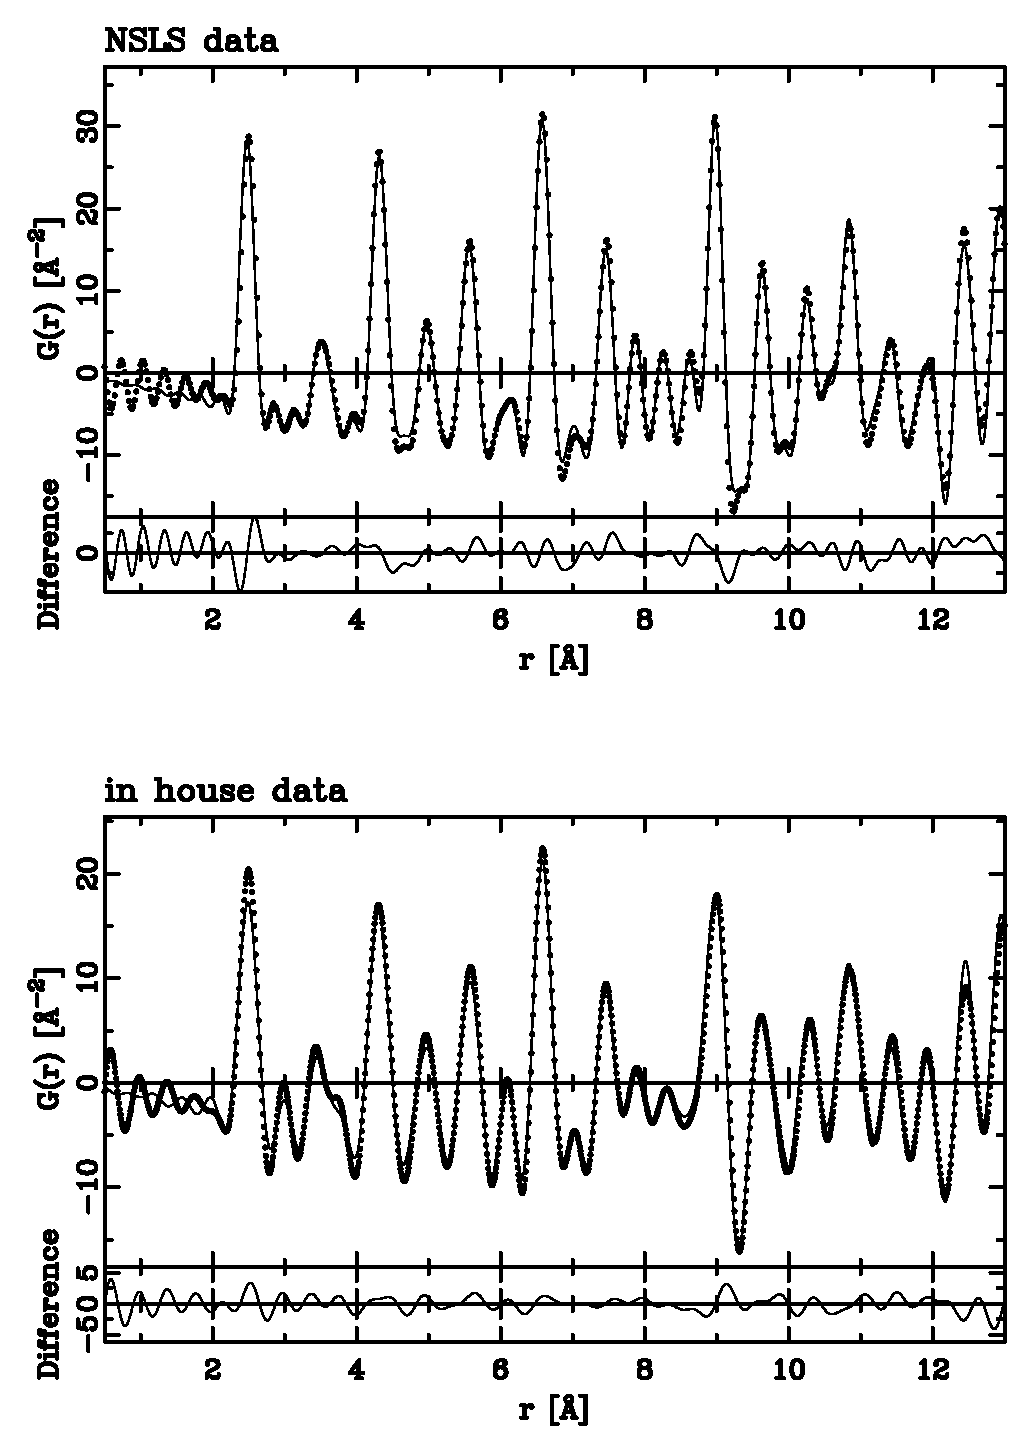
\includegraphics[scale=0.65, angle=0]{exa.3.eps}
   \caption[Result of PDF refinement of two data sets of $Ni$]
           {Result of PDF refinement of two data sets of $Ni$.
            The solid line is the calculated PDF, the filled circles are
            the data. The top panel shows synchrotron (NSLS) data,
            the bottom panel shows data from a in house X-ray source.
            A difference curve is plotted below the data.}
   \label{exa_fig3}
\end{figure}

\footnotesize
\begin{MacVerbatim}
      1 reset
      2 read stru,ni.stru
      3 read data,x,22.0,0.0,ni-nsls.data
      4 read data,x,16.0,0.0,ni-inhs.data
      5 #
      6 range 1,0.5,13.0
      7 range 2,0.5,13.0
      8 #
      9 par dsca[1]=p[10],1.0
     10 par dsca[2]=p[11],1.0
     11 par qsig[1]=p[12],1.0
     12 par qsig[2]=p[13],1.0
     13 #
     14 par delt[1]=p[14],1.0
     15 #
     16 p[10]=1.50
     17 p[11]=1.00
     18 p[12]=0.03
     19 p[13]=0.03
     20 p[14]=0.10
\end{MacVerbatim}
\normalsize

\noindent The first two lines are as before, resetting {\it
PDFFIT} and reading the structure file. Now we need to issue a
{\tt read} command for each data set. Note the different file
names and values for $Q_{max}$ in lines 3 and 4. There are two
data set dependent parameters, the scaling factor $f_{s}$ and the
resolution factor $\sigma_{Q}(s)$. One refinement parameter is
assigned to each one for each of the two data sets (lines 9--12).
Note that in previous examples we have used the scale factor
$f_{p}$ corresponding to the structural phase $p$. In cases where
we have only {\it one} phase and {\it one} data set we are free to
choose which scale factor to refine. Now the scale factors related
to the different data sets must be used. The starting values for
the different defined refinement parameters are set in lines
16--20.

\footnotesize
\begin{MacVerbatim}
     21 #
     22 ###########################################################
     23 # Refining lattice parameters and thermal factors
     24 ###########################################################
     25 #
     26 par lat[1]=p[1],1.0
     27 par lat[2]=p[1],1.0
     28 par lat[3]=p[1],1.0
     29 #
     30 do i[1]=1,n[1]
     31   par u[1,i[1]]=p[2],1.0
     32   par u[2,i[1]]=p[2],1.0
     33   par u[3,i[1]]=p[2],1.0
     34 enddo
     35 #
     36 p[1]=lat[1]
     37 p[2]=u[1,1]
     38 #
     39 ###########################################################
     40 # Running the refinement and saving results
     41 ###########################################################
     42 #
     43 run
     44 #
     45 save pdf,1,ni-nsls.calc
     46 save pdf,2,ni-inhs.calc
     47 save dif,1,ni-nsls.dif
     48 save dif,2,ni-inhs.dif
     49 save stru,1,ni_ref.stru
     50 save res,ni_ref.out
\end{MacVerbatim}
\normalsize

\noindent In this last part of the macro, we define refinement
parameters for the lattice parameters $a=b=c$ and the isotropic
thermal factor for the $Ni$ atom. This is identical to the quick
example given in chapter \ref{quick}, the only difference is that
one needs to save the calculated PDF and the difference between
observed and calculated PDF for each data set separately (lines
45--48). The results for the synchrotron as well as the in-house
data can be seen in Figure \ref{exa_fig3}. Note that {\it PDFFIT}
outputs only the total R-value of the refinement. Individual
R-values for the different data sets or for a specific region in
$r$ can be obtained using the {\it PDFFIT} function {\tt rval}
(see section \ref{func}).

%------------------------------------------------------------------------
